\documentclass[tikz,border=2pt]{standalone}
\usepackage{amsmath,amssymb}
\usepackage{tikz}
\usetikzlibrary{arrows.meta}

\begin{document}
% Two-phase method: Phase I drives the artificial variables to zero (finding a feasible
% corner); Phase II restarts from that corner with the real objective.
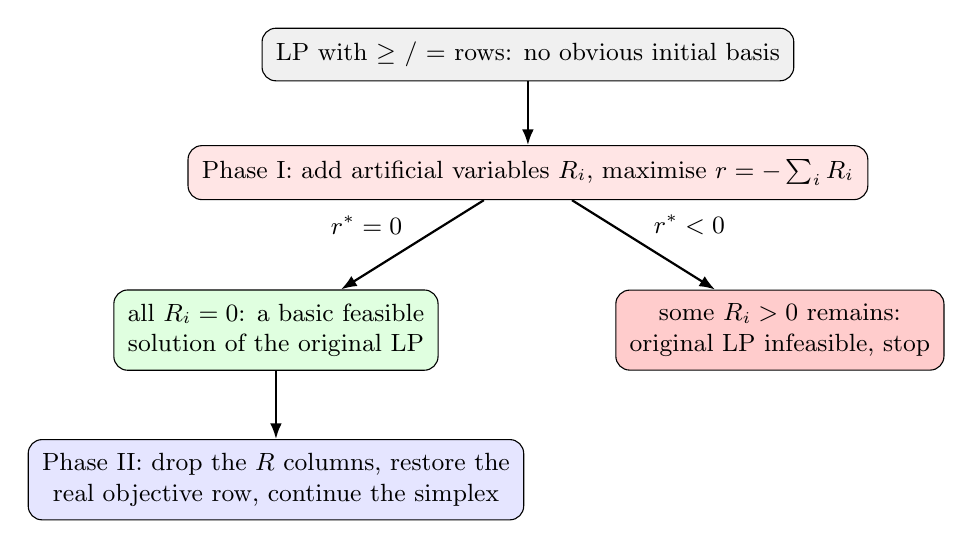
\begin{tikzpicture}[every node/.style={font=\small}, >={Latex[length=2mm]}, bx/.style={draw, rounded corners=5pt, inner sep=5pt, align=center}]
	\node[bx, fill=gray!12] (a) at (0,0) {LP with $\ge$ / $=$ rows: no obvious initial basis};
	\node[bx, fill=red!10] (b) at (0,-1.5) {Phase I: add artificial variables $R_i$, maximise $r=-\sum_iR_i$};
	\node[bx, fill=green!12] (c) at (-3.2,-3.5) {all $R_i=0$: a basic feasible\\ solution of the original LP};
	\node[bx, fill=red!20] (d) at (3.2,-3.5) {some $R_i>0$ remains:\\ original LP infeasible, stop};
	\node[bx, fill=blue!10] (e) at (-3.2,-5.4) {Phase II: drop the $R$ columns, restore the\\ real objective row, continue the simplex};
	\draw[->, thick] (a) -- (b);
	\draw[->, thick] (b) -- (c) node[midway, above left, font=\small] {$r^\ast=0$};
	\draw[->, thick] (b) -- (d) node[midway, above right, font=\small] {$r^\ast<0$};
	\draw[->, thick] (c) -- (e);
	\end{tikzpicture}
\end{document}
